%%%%%%%%%%%%%%%%%%%%%%%%%%%%%%%%%%%%%%%%%%%%%%%%%%%%%%%%%%%%%%%%%%%%%%%%
%     LaTeX source code to approximate a NIST Technical report
%	  Instructions for authors: tinyurl.com/techpubsnist
%	DOI watermark will be added on final PDF
% 	Developed by K. Miller, kmm5@nist.gov
%	Last updated: 10-Oct-2017
%%%%%%%%%%%%%%%%%%%%%%%%%%%%%%%%%%%%%%%%%%%%%%%%%%%%%%%%%%%%%%%%%%%
\documentclass[12pt]{article}
\usepackage{adjustbox}
\usepackage{amsmath}
\usepackage{amsfonts}   % if you want the fonts
\usepackage{amssymb}    % if you want extra symbols
\usepackage{graphicx}   % need for figures
\usepackage{xcolor}
\usepackage{bm}
\usepackage{secdot}		
\usepackage{mathptmx}
\usepackage{multicol}
\usepackage{float}
\usepackage[utf8]{inputenc}
\usepackage{textgreek}
\usepackage{textcomp}
\usepackage[hang,flushmargin,bottom]{footmisc} % footnote format
\usepackage{siunitx} % Formats the units and values
\usepackage{titlesec}
\usepackage{tikz}
\titleformat{\section}{\normalsize\bfseries}{\thesection.}{1em}{}	% required for heading numbering style
\titleformat*{\subsection}{\normalsize\bfseries}

\usepackage{tocloft}	% change typeset, titles, and format list of appendices/figures/tables
\renewcommand{\cftdot}{}	
\renewcommand{\contentsname}{Table of Contents}
\renewcommand{\cftpartleader}{\cftdotfill{\cftdotsep}} % for parts
\renewcommand{\cftsecleader}{\cftdotfill{\cftdotsep}}
\renewcommand\cftbeforesecskip{\setlength{4pt}{}}
\addtolength{\cftfignumwidth}{1em}
\renewcommand{\cftfigpresnum}{\figurename\ }
\addtolength{\cfttabnumwidth}{1em}
\renewcommand{\cfttabpresnum}{\tablename\ }
\setlength{\cfttabindent}{0in}    %% adjust as you like
\setlength{\cftfigindent}{0in}

\usepackage{enumitem}         % to control spacing between bullets/numbered lists

\usepackage[numbers,sort&compress]{natbib} % format bibliography
\renewcommand{\bibsection}{}
\setlength{\bibsep}{0.0pt}

\usepackage[hidelinks]{hyperref} % hyperref package & removing outline from links

\usepackage{epstopdf} % converting EPS figure files to PDF

\usepackage{fancyhdr, lastpage}	% formatting document, calculating number of pages, formatting headers
\setlength{\topmargin}{-0.5in}
\setlength{\headheight}{39pt}
\setlength{\oddsidemargin}{0.25in}
\setlength{\evensidemargin}{0.25in}
\setlength{\textwidth}{6.0in}
\setlength{\textheight}{8.5in}

\usepackage{caption} % required for Figure labels
\captionsetup{font=small,labelfont=bf,figurename=Fig.,labelsep=period,justification=raggedright}

%%%%%%%%%%% !!!!!! REQUIRED - FILL OUT METADATA HERE !!!!!!!! %%%%%%%%%%%%%%
%  	Report Number - fill in Report Number sent to you (see info below)
%   DOI Statement - fill in DOI sent to you
%   Month Year - fill in Month and Year of Publication
%%%%%%%%%%%%%%%%%%%%%%%%%%%%%%%%%%%%%%%%%%%%%%%%%%%%%%%%%%%%%%%%%%%%%%%%%%%%%%%%%%%%%%
\newcommand{\pubnumber}{XXXX}
\newcommand{\DOI}{https://doi.org/10.6028/NIST.TN.XXXX}
\newcommand{\monthyear}{Month Year}
%%%%%%%%%%%%%%%%%%%%%%%%%%%%%%%%%%%%%%%%%%%%%%%%%%%%%%%%%%%%%%%%%%%%
%   	BEGIN DOCUMENT
%%%%%%%%%%%%%%%%%%%%%%%%%%%%%%%%%%%%%%%%%%%%%%%%%%%%%%%%%%%%%%%%%%%%
\begin{document}
	\urlstyle{rm} % Format style of \url
	
%%%%%%%%%%%%%%%%%%%%%%%%%%%%%%%%%%%%%%%%%%%%%%%%%%%%%%%%%%%%%%%%%%%%
%   Cover Page is REQUIRED and must contain the information
%	displayed here, at a minimum. Additional artwork may be included
%	(e.g., official project/conference logo, etc.).
%	Pub Number automated based on metadata
%%%%%%%%%%%%%%%%%%%%%%%%%%%%%%%%%%%%%%%%%%%%%%%%%%%%%%%%%%%%%%%%%%%%
	\begin{titlepage}
		\begin{flushright}
%%%%%%%%%%%%%%%%%%%%%%%%%%%%%%%%%%%%%%%%%%%%%%%%%%%%%%%%%%%%%%%%%%%%
% 	Automated based on metadata - delete if not applicable
%%%%%%%%%%%%%%%%%%%%%%%%%%%%%%%%%%%%%%%%%%%%%%%%%%%%%%%%%%%%%%%%%%%%
\LARGE{\textbf{NIST Technical Note \pubnumber}}\\
\vfill
%%%%%%%%%%%%%%%%%%%%%%%%%%%%%%%%%%%%%%%%%%%%%%%%%%%%%%%%%%%%%%%%%%%%
%	Title
%%%%%%%%%%%%%%%%%%%%%%%%%%%%%%%%%%%%%%%%%%%%%%%%%%%%%%%%%%%%%%%%%%%%
\Huge{\textbf{Measurement of the Flow Resistance of Vegetation}}\\
\vfill
%%%%%%%%%%%%%%%%%%%%%%%%%%%%%%%%%%%%%%%%%%%%%%%%%%%%%%%%%%%%%%%%%%%%
%	Authors - add complete list of authors, affiliations will be
%   added on title page
%%%%%%%%%%%%%%%%%%%%%%%%%%%%%%%%%%%%%%%%%%%%%%%%%%%%%%%%%%%%%%%%%%%%
\large Ryan Falkenstein-Smith\\
\large Kevin McGrattan\\
\large Marco Fernandez \\
\vfill
%%%%%%%%%%%%%%%%%%%%%%%%%%%%%%%%%%%%%%%%%%%%%%%%%%%%%%%%%%%%%%%%%%%%
%	The DOI is automated based on metadata.	
%%%%%%%%%%%%%%%%%%%%%%%%%%%%%%%%%%%%%%%%%%%%%%%%%%%%%%%%%%%%%%%%%%%%
\normalsize This publication is available free of charge from:\\
\DOI\\
\vfill
%%%%%%%%%%%%%%%%%%%%%%%%%%%%%%%%%%%%%%%%%%%%%%%%%%%%%%%%%%%%%%%%%%%%
%	NIST LOGO - keep as-is
%%%%%%%%%%%%%%%%%%%%%%%%%%%%%%%%%%%%%%%%%%%%%%%%%%%%%%%%%%%%%%%%%%%%


\includegraphics[width=0.3\linewidth]{NIST-logo.eps}\\


\end{flushright}
\end{titlepage}
\begin{titlepage}
%%%%%%%%%%%%%%%%%%%%%%%%%%%%%%%%%%%%%%%%%%%%%%%%%%%%%%%%%%%%%%%%%%%%
%	Title Page is REQUIRED
%%%%%%%%%%%%%%%%%%%%%%%%%%%%%%%%%%%%%%%%%%%%%%%%%%%%%%%%%%%%%%%%%%%%
\begin{flushright}
%%%%%%%%%%%%%%%%%%%%%%%%%%%%%%%%%%%%%%%%%%%%%%%%%%%%%%%%%%%%%%%%%%%%
%   Publication Series & Number - automated
%%%%%%%%%%%%%%%%%%%%%%%%%%%%%%%%%%%%%%%%%%%%%%%%%%%%%%%%%%%%%%%%%%%%
\LARGE{\textbf{NIST Technical Note \pubnumber}}\\
\vfill
%%%%%%%%%%%%%%%%%%%%%%%%%%%%%%%%%%%%%%%%%%%%%%%%%%%%%%%%%%%%%%%%%%%%
%	Title
%%%%%%%%%%%%%%%%%%%%%%%%%%%%%%%%%%%%%%%%%%%%%%%%%%%%%%%%%%%%%%%%%%%%
\Huge{\textbf{Measurement of the Flow Resistance of Vegetation}}\\
\vfill
%%%%%%%%%%%%%%%%%%%%%%%%%%%%%%%%%%%%%%%%%%%%%%%%%%%%%%%%%%%%%%%%%%%%
%	Author Order and Grouping. Always identify the primary author/creator first (s/he does not have to be a NIST author). For publications with multiple authors, group authors by their organizational affiliation. The organizational groupings and the names within each grouping should generally be ordered by decreasing level of contribution.
%	For non-NIST authors, list their city and state below their organization name.
%	For NIST authors, include the Division and Laboratory names (but do not include their city and state).
%%%%%%%%%%%%%%%%%%%%%%%%%%%%%%%%%%%%%%%%%%%%%%%%%%%%%%%%%%%%%%%%%%%%
\normalsize Ryan Falkenstein-Smith\\
Kevin McGrattan\\
Marco Fernandez\\
\textit{Fire Research Division}\\
\textit{Engineering Laboratory}\\
\vspace{12pt}
\vfill
%%%%%%%%%%%%%%%%%%%%%%%%%%%%%%%%%%%%%%%%%%%%%%%%%%%%%%%%%%%%%%%%%%%%
%   DOI Statement - automated
%%%%%%%%%%%%%%%%%%%%%%%%%%%%%%%%%%%%%%%%%%%%%%%%%%%%%%%%%%%%%%%%%%%%
\normalsize This publication is available free of charge from:\\
\DOI\\
\vfill
%%%%%%%%%%%%%%%%%%%%%%%%%%%%%%%%%%%%%%%%%%%%%%%%%%%%%%%%%%%%%%%%%%%%
%   Date - Month and Year - automated
%%%%%%%%%%%%%%%%%%%%%%%%%%%%%%%%%%%%%%%%%%%%%%%%%%%%%%%%%%%%%%%%%%%%
\normalsize \monthyear
\vfill
%%%%%%%%%%%%%%%%%%%%%%%%%%%%%%%%%%%%%%%%%%%%%%%%%%%%%%%%%%%%%%%%%%%%
%  Department of Commerce LOGO - leave as-is
%%%%%%%%%%%%%%%%%%%%%%%%%%%%%%%%%%%%%%%%%%%%%%%%%%%%%%%%%%%%%%%%%%%%	


\includegraphics[width=0.18\linewidth]{DoC-logo.eps}\\
\vfill
%%%%%%%%%%%%%%%%%%%%%%%%%%%%%%%%%%%%%%%%%%%%%%%%%%%%%%%%%%%%%%%%%%%%
%  Department of Commerce & NIST Leadership
%	will be updated as changes occur
%%%%%%%%%%%%%%%%%%%%%%%%%%%%%%%%%%%%%%%%%%%%%%%%%%%%%%%%%%%%%%%%%%%%
\footnotesize U.S. Department of Commerce\\
\textit{Wilbur L. Ross, Jr., Secretary}\\
\vspace{10pt}
National Institute of Standards and Technology\\
\textit{Walter Copan, NIST Director and Undersecretary of Commerce for Standards and Technology}
\end{flushright}
\end{titlepage}

\begin{titlepage}
%%%%%%%%%%%%%%%%%%%%%%%%%%%%%%%%%%%%%%%%%%%%%%%%%%%%%%%%%%%%%%%%%%%%
%   Disclaimer/CODEN page - required
%%%%%%%%%%%%%%%%%%%%%%%%%%%%%%%%%%%%%%%%%%%%%%%%%%%%%%%%%%%%%%%%%%%%
\begin{flushright}
\footnotesize  Certain commercial entities, equipment, or materials may be identified in this document in order to describe an experimental procedure or concept adequately. Such identification is not intended to imply recommendation or endorsement by the National Institute of Standards and Technology, nor is it intended to imply that the entities, materials, or equipment are necessarily the best available for the purpose.\\
\vfill
%%%%%%%%%%%%%%%%%%%%%%%%%%%%%%%%%%%%%%%%%%%%%%%%%%%%%%%%%%%%%%%%%%%%
%   This secton automated - do not change
%%%%%%%%%%%%%%%%%%%%%%%%%%%%%%%%%%%%%%%%%%%%%%%%%%%%%%%%%%%%%%%%%%%%
\normalsize \textbf{National Institute of Standards and Technology Technical Note \pubnumber\\
Natl. Inst. Stand. Technol. Tech. Note \pubnumber, \pageref{LastPage} pages (\monthyear)} \\
\textbf{CODEN: NTNOEF}\\
\vspace{12pt}
\textbf{This publication is available free of charge from: \DOI}
\vfill
\end{flushright}
\end{titlepage}
%%%%%%%%%%%%%%%%%%%%%%%%%%%%%%%%%%%%%%%%%%%%%%%%%%%%%%%%%%%%%%%%%%%%
%   Start front matter - page number starts with "i"
%%%%%%%%%%%%%%%%%%%%%%%%%%%%%%%%%%%%%%%%%%%%%%%%%%%%%%%%%%%%%%%%%%%%
\pagenumbering{roman}
\section*{Abstract}
\normalsize This report documents a series of experiments carried out on a variety of vegetation canopy to determine their resistance to airflow. The objective of each experiment was a follows: Experiment 1) determine the vegetations' projected area using standard photography equipment and image analysis software, Experiment 2) measure the pressure loss across vegetation canopy while exposed to steady wind speeds in an open circuit wind tunnel, and Experiment 3) quantify the total volume of the vegetation canopy using a water displacement technique. The results obtained from these experiments were combined to calculate the drag coefficient of the vegetation canopy and provided further insight into the relationship between the vegetations' geometric properties and resistance to airflow. Furthermore, specific parameters determined from the experiments were incorporated into well-established hydraulic resistance models of configurations with similar geometry (i.e., tube banks) to validate the calculated drag coefficients of the vegetation canopy. \\
\section*{Key words}
\normalsize Vegetation Canopy; Drag Coefficient; Wind Tunnel; Tube Banks.\\
\pagebreak
%%%%%%%%%%%%%%%%%%%%%%%%%%%%%%%%%%%%%%%%%%%%%%%%%%%%%%%%%%%%%%%%%%%%
%   Table of Contents is required
% 	List of Tables & Figures required if more than 5 tables/figures
%%%%%%%%%%%%%%%%%%%%%%%%%%%%%%%%%%%%%%%%%%%%%%%%%%%%%%%%%%%%%%%%%%%%
\begin{center}
	\tableofcontents
	\listoftables
	\listoffigures
\end{center}
\pagebreak

\pagenumbering{arabic}
\normalsize 


\section{Introduction}
\label{sec:intro}

The Fire Research Division of the National Institute of Standards and Technology (NIST) has developed several numerical models to predict the behavior of fires within buildings. One of the models, a computational fluid dynamics (CFD) code called the Fire Dynamics Simulator (FDS)~\cite{FDS_Tech_Guide}, has been extended to model fires in the wildland-urban interface (WUI). One crucial component of this type of modeling is a proper treatment of wind-driven flow through vegetation. The objective of the experiments described in this report is to measure the drag coefficient of an empirical sub-model appropriate for CFD.

Measurements of this type have been performed by other researchers~\cite{Cao2012,Jalonen2014,Mayhead1973,Gillies2002,Ishikawa2006}, most of whom used wind tunnels of various sizes. In most cases, a single plant or small tree was positioned within the tunnel and the resistance force measured. However, such a measurement is not readily applicable to a CFD model which does not necessarily consider the tree as a whole but rather as a volume occupied by subgrid-scale objects that decrease momentum in the grid cells that they occupy. Some plants might be smaller than a characteristic grid cell, and some trees might be larger, but in either case, these objects are just momentum sinks within individual grid cells that require some sort of drag coefficient that is appropriate to the local conditions. That is, it is not appropriate to talk about the ``free stream velocity'' within a CFD model, as the velocity changes from cell to cell.


\section{Model Development}
\label{ssec:headingscap}

The objective of the experiments described in this report is to measure a drag coefficient appropriate for an empirical model of wind resistance by ``bulk'' vegetation. This model is to be used within a CFD model where vegetation is taken as a  collection of subgrid-scale solid particles whose mass, size, and shape are characterized by a handful of parameters that can be determined with field measurements. The term ``bulk'' vegetation stresses the fact that the objective is not to consider the drag exerted by a single tree or shrub, but rather a characteristic volume filled with a random collection of leaves, pine needles, etc., as shown in the simple schematic of Fig.~\ref{fig:Canopymod}. This volume can be thought of as a grid cell in the CFD model that has an average flow speed, $U$, and gas density, $\rho$.
\begin{figure}[!ht]
	\centering 	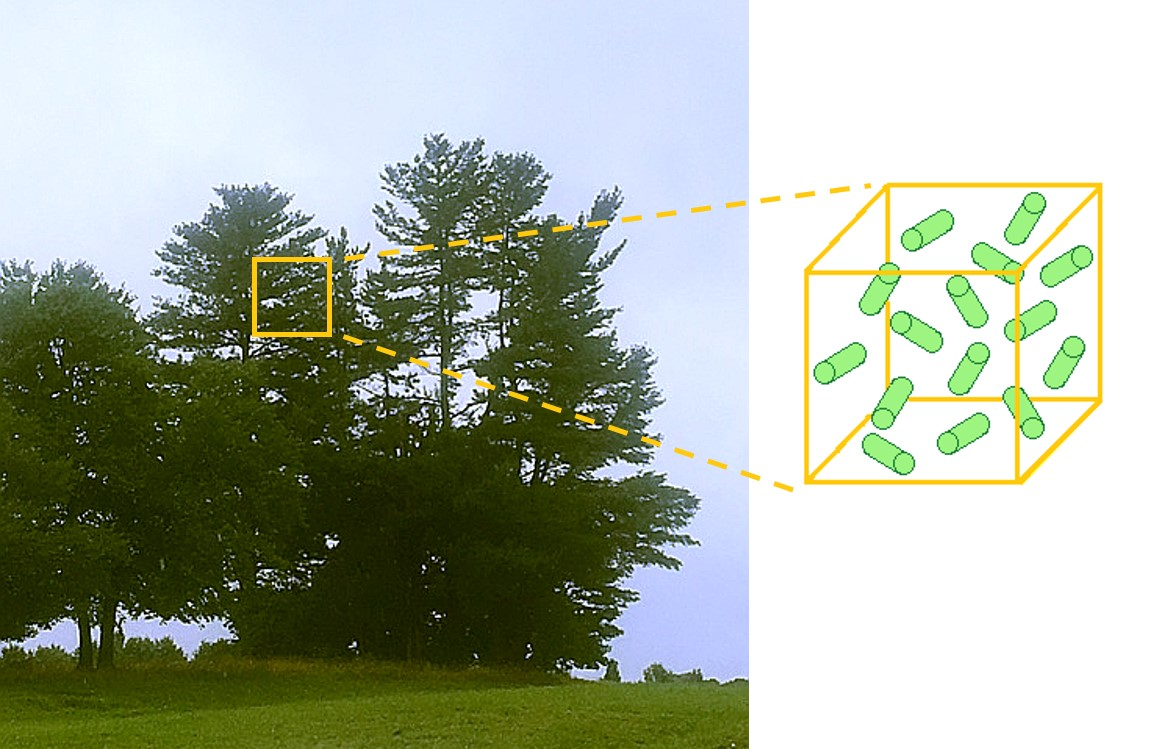
\includegraphics[width=1.0\linewidth]{Picture1.jpg}
	\caption{Vegetation translation to multi-component model}
	\label{fig:Canopymod}
\end{figure}
The force per unit volume added to the momentum equation is given by the expression:
\begin{equation}
\label{eq:DragForce}
F_{\mathrm{D}} = \frac{1}{V} \, \frac{\rho}{2} \, \sum_{i=1}^N  C_{\mathrm{D}} \, A_{\mathrm{p},i} \, {U}^2 
\end{equation}
where $V$ is the volume of the grid cell, $A_{\mathrm{p},i}$ is the projected area of the $i$th vegetative component, and $C_{\mathrm{D}}$ is a drag coefficient which is taken as a constant. Similar configurations have already been been adapted in numerical investigations~\cite{Pimont2009, Dupont2008}.

Equation~(\ref{eq:DragForce}) can be recast in an equivalent form that is more useful for describing vegetation drag~\cite{Mueller2014}:
\begin{equation}
\label{eq:DragForcea}
F_{\mathrm{D}}  = \frac{\rho}{2} C_{\mathrm{D}} \, C_{\mathrm{s}} \, \beta \, \sigma \, U^2
\end{equation}
where $C_{\mathrm{s}}$ is a characteristic shape factor defined in this case as the ratio of the projected area to surface area of each vegetative component, $\beta$ is the ratio of the volume occupied by vegetation to the control volume, $V$, and $\sigma$ is the surface area to volume ratio of each vegetative component. Some of the terms are difficult to measure, such as the shape factor and surface to volume ratio. However, these terms may be combined to form a parameter that resembles an absorption coefficient:
\begin{equation}
\label{eq:WhiteFraction} 
\kappa = C_{\mathrm{s}} \, \beta \, \sigma 
\end{equation}
that can be determined by measuring the projected area of light passing a distance $L$ through the vegetation. The relative area of light, or ``white fraction'', is defined by the relation:
\begin{equation}\label{eq:WhiteFraction}
W = {\rm e}^{-\kappa L}
\end{equation}
In the experiments, the cross section of a small wind tunnel is filled with various amounts of various types of vegetation and the drag coefficient is determined for the following simplified model:
\begin{equation}\label{eq:Pressure}
F_{\mathrm{D}} \equiv \frac{\Delta P}{L}  = \frac{\rho}{2} \, C_{\mathrm{D}} \, \kappa \, U^2
\end{equation}



\section{Description of Experiments}
\label{sec:Experiments}
\subsection{Vegetation Preparation and Investigation Procedure}
\label{ssec:headingscap}

The vegetation chosen for this work was a Bakers Blue Spruce, an Evergreen Distylium, a Gold Rider Leyland Cypress, a Kimberley Queen Fern, a Blue Shag Eastern White Pine, and a Robin Red Holly. Each vegetation sample was chosen for this study based on their local availability. Leaf shapes of the vegetation samples included needle, elliptic, scale, and ovate shapes.

To mimic a segment of vegetation canopy similarly investigated in a numerical simulation, samples were cut  into 0.5 m x 0.5 m x 0.5 m cubes using a cubic guiding frame then to a thin steel plate (Fig. \ref{fig:Sampleprep}). The 0.5 m x 0.5 m cross-section of the segmented vegetation canopy fully occupied the cross-section of the wind tunnel forcing the flow to move through the vegetation as opposed to around it. The center of each cubic vegetation sample's side was marked on the base plate to better the perpendicular alignment of the vegetation to the flow when placed in the wind tunnel. To easily distinguish the front, back, left, and right side of the cube-shaped vegetation, each side was designated a name of position A (PA), position B (PB), position C (PC), or position D (PD) (Fig. \ref{fig:Vegpos}). After its initial cut, image analysis, wind tunnel measurements, and water displacement testing were conducted in subsequent order. In some cases, additional cuts were made to certain samples at the conclusion of the experimental procedure (Fig. \ref{fig:flowchart}). The decision to make additional cuts made to the vegetation samples mainly depended on the lively hood of the particular sample after an iteration in the experimental procedure. In the case of the Bakers Blue Spruce, Gold Rider Leyland Cypress, and Robin Red Holly, four iterative cuts were made with the final cut being the removal of all leaves from the vegetation.

\begin{figure} [h]
	\centering 	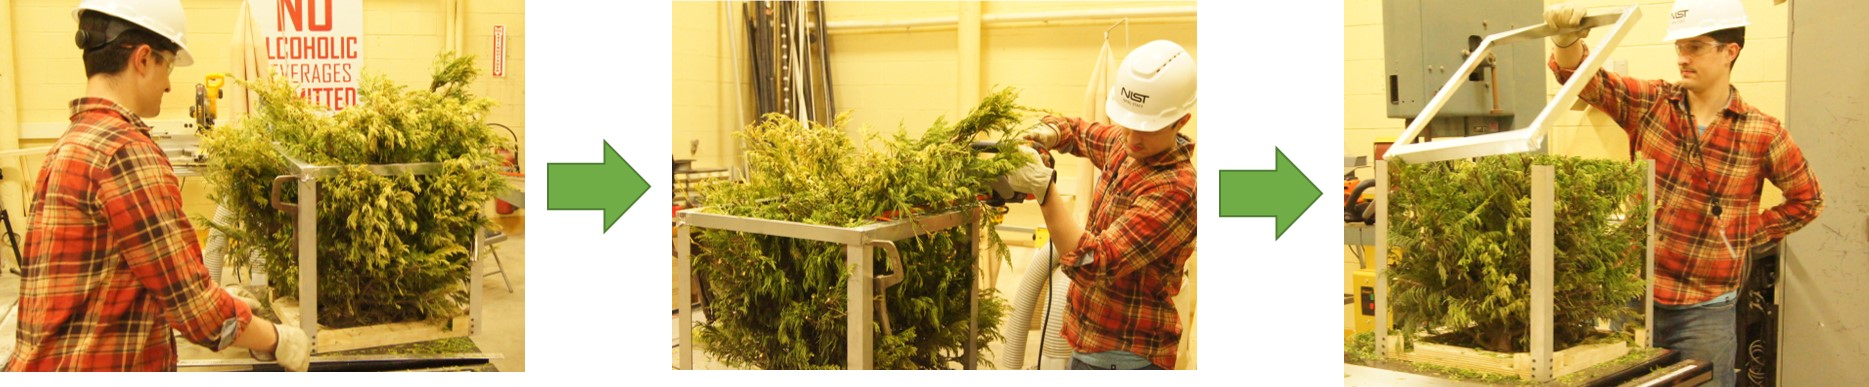
\includegraphics[width=1.0\linewidth]{Picture2.jpg}
	\caption{Cutting procedure of vegetation samples}
	\label{fig:Sampleprep}
\end{figure}

\begin{figure} [!]
	\centering 	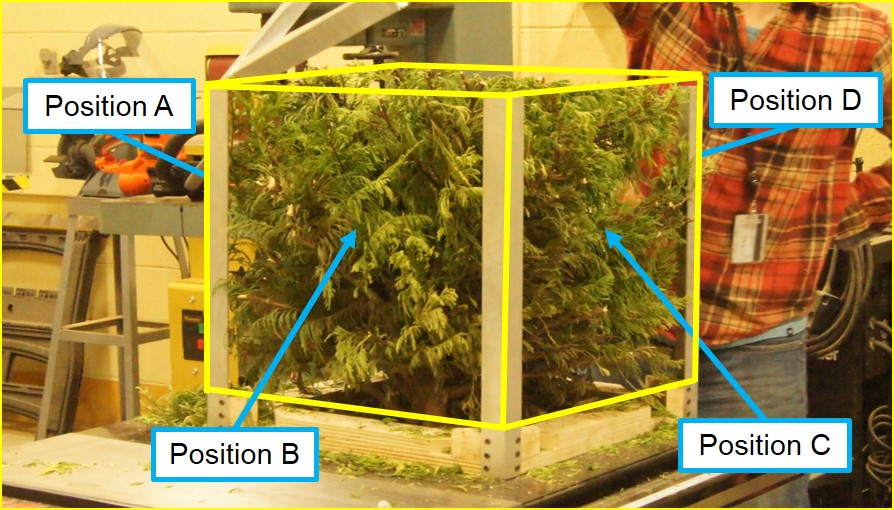
\includegraphics[width=1.0\linewidth]{Picture3.jpg}
	\caption{Prepared vegetation sample's designated orientation}
	\label{fig:Vegpos}
\end{figure}

\begin{figure} [!]
	\centering 	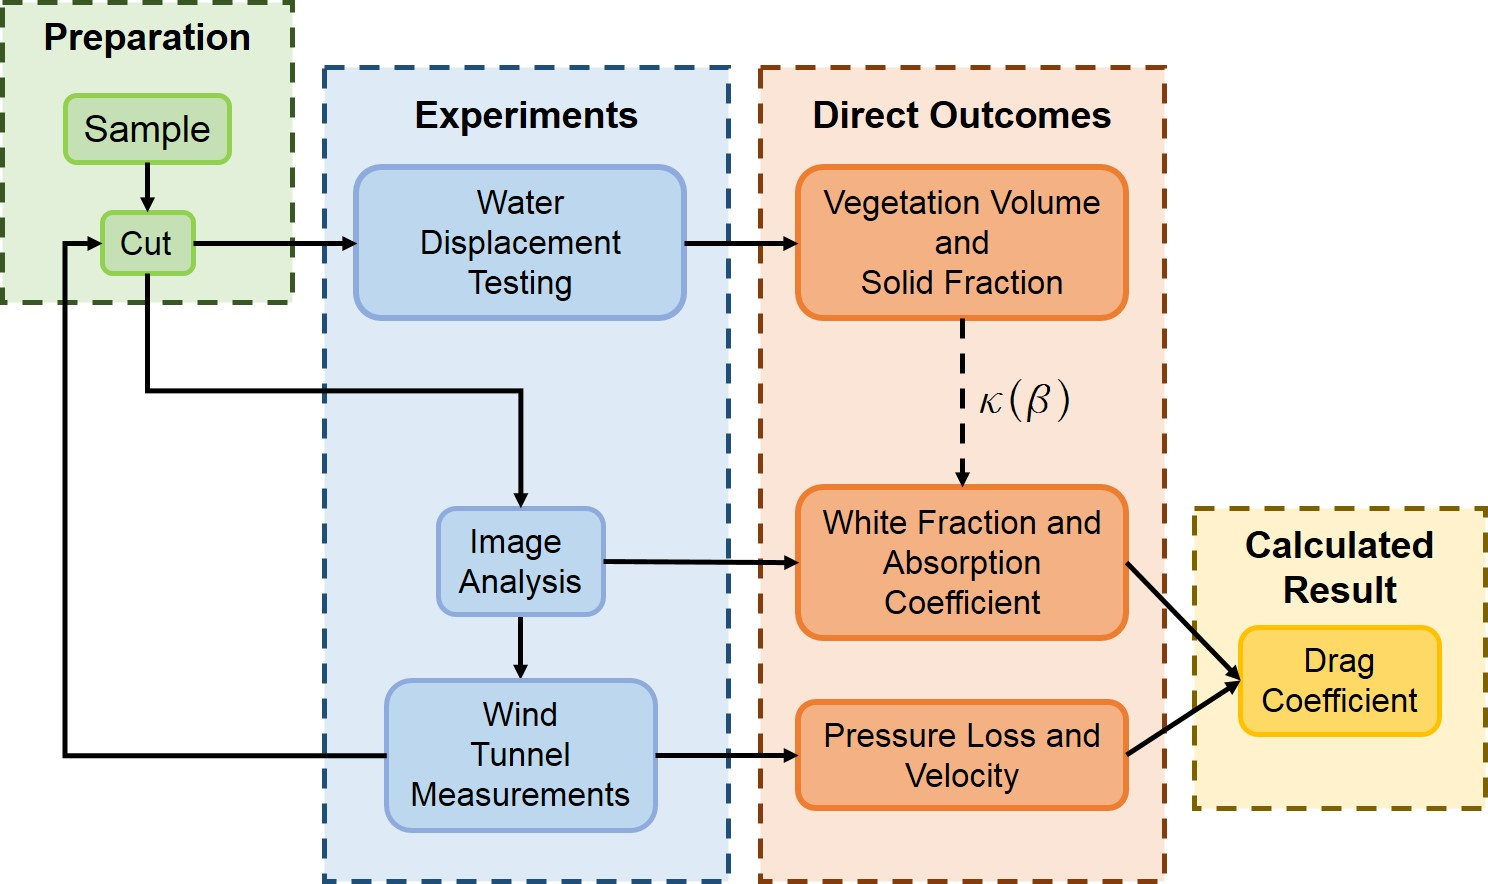
\includegraphics[width=1.0\linewidth]{Picture4.jpg}
	\caption{Flowchart of experimental procedures and their respective outcomes}
	\label{fig:flowchart}
\end{figure}



\subsection{Image Analysis to Determine the Absorption Coefficient }
\label{ssec:headingscap}

The absorption coefficient of the vegetation samples were determined from the free area fraction ($W$) of the projected area of the sample. After segmenting the vegetation, the sample was placed on a table located between a large white backdrop and a 0.5 m x 0.5 m cardboard frame (Fig. \ref{fig:ImgAnaly}). The cardboard frame dimensions were the same as cross-section dimensions within the wind tunnel, providing an accurate representation of the vegetation's projected area when placed within the tunnel. For each sample cut, an image of each cubic sample's sides was captured. All images were captured using a Nikon D5600 camera placed on a tripod located approximately 3.6 \si{m} away from the frontal plane of the vegetation sample. In order to identify smaller areas of white space, the white backdrop was illuminated using a collection of incandescent and LED lights.\\

\begin{figure} [h]
	\centering 	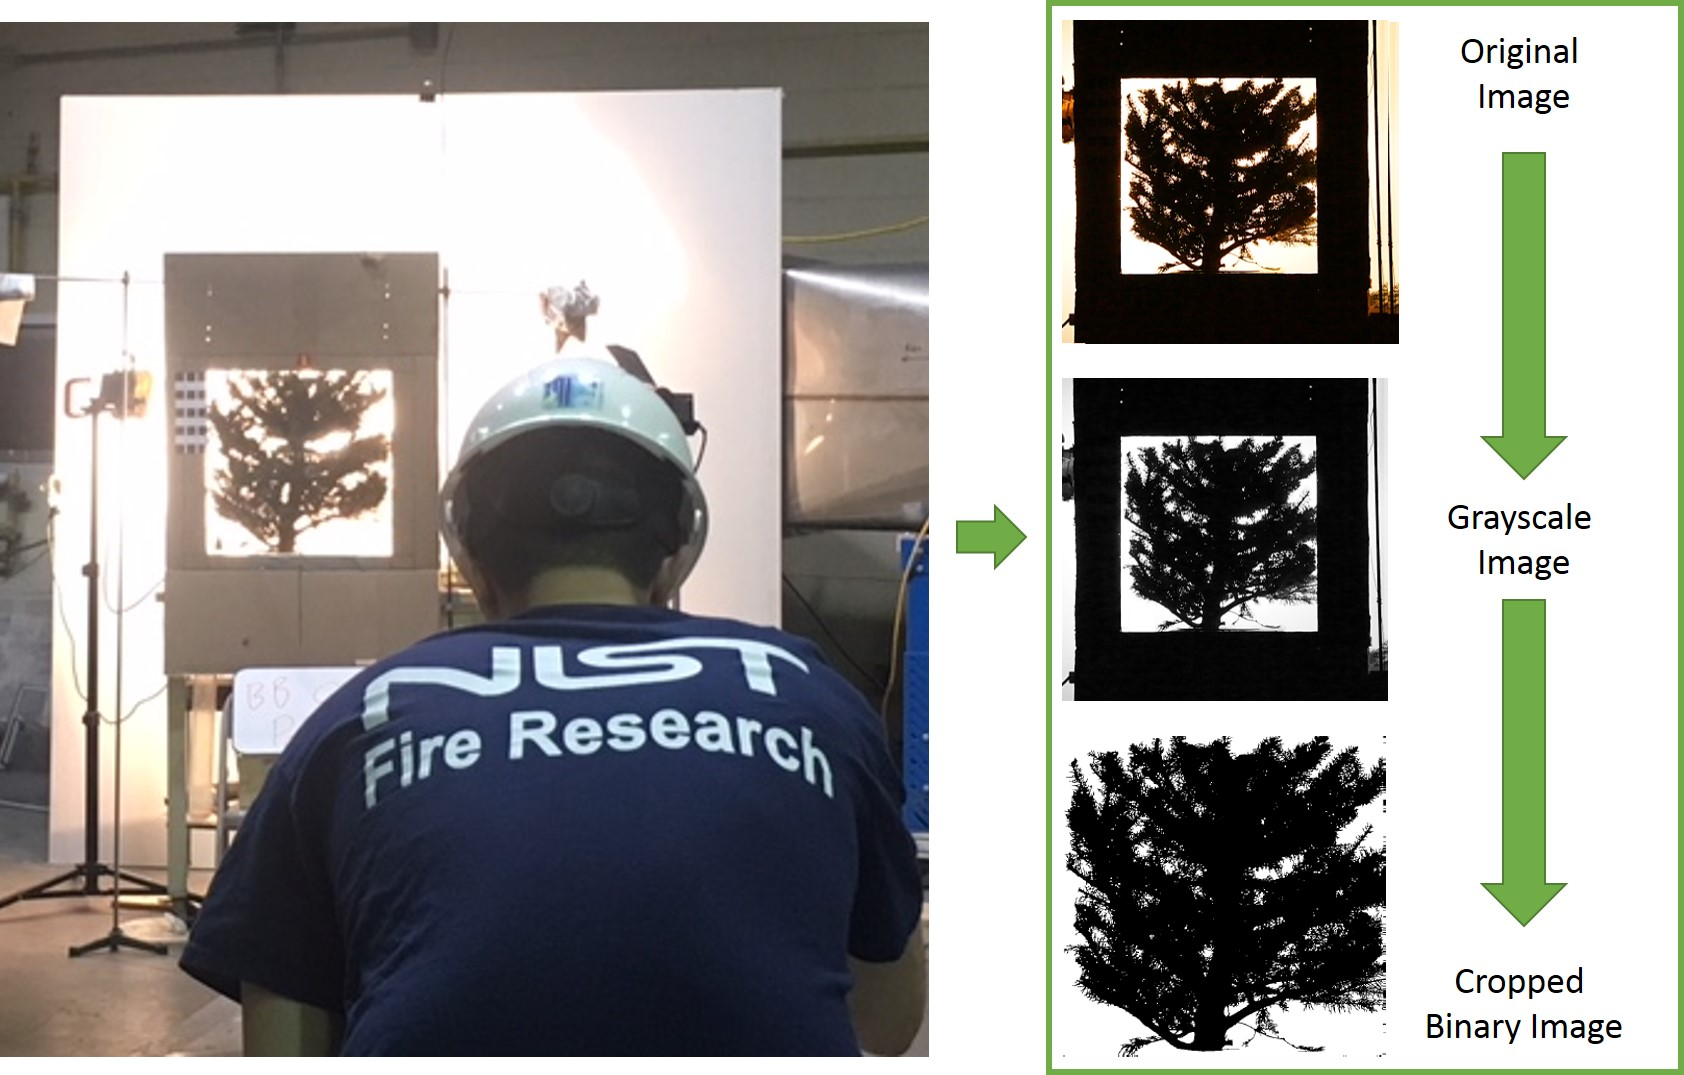
\includegraphics[width=1.0\linewidth]{Picture5.jpg}
	\caption{Setup for photographing vegetation samples (left) and the post-processing procedure for analyzing images (right)}
	\label{fig:ImgAnaly}
\end{figure}

\indent After photographing the projected area of vegetation, the captured images were processed using MATLAB's Image Processing Toolbox. Imported images were first cropped within the cardboard frame to eliminate nonvegetative substances and to exclusively evaluate the projected vegetation area. The obtained colored image was converted into a grey scale then binary (black and white) image using a pre-set threshold level. Once converted into a binary image, a pixel count was conducted to determine the free area fraction of the vegetation. After obtaining the free area fractions for each position of the vegetation sample, the average free area fraction was calculated by averaging the parallel sides of the cubic vegetation.\\
\indent An uncertainty analysis was also conducted on the imaging process. Before using segmented vegetation samples, objects of known projected areas were photographed using the same imaging setup. It was found that with each object, the calculated free area fraction varied from the true value by 1\%. Therefore, the error of the free area fraction values was assumed to be 1\%. The uncertainty of each determined free area fraction also accounted for the averaged value using propagation of error.

\subsection{Wind Tunnel Experiments to Measure the Pressure Loss Across Vegetation}
\label{ssec:headingscap}

Pressure loss measurements were obtained in a wind tunnel test section with a cross-sectional area of 0.5 m x 0.5 m and a length of 2 \si{m}. Differential pressure was measured in two sections: 1) upstream using a Rosemont 485 Annubar Primary Element and 2) downstream between two pressure taps placed approximately 5 cm away from the vegetation sample  (Fig. \ref{fig:Windtun}). The differential pressure was specifically measured using two MKS Baratron Type 220D Pressure Transducer with a range of 0 to 1 torr (133 Pa). The air flow was provided by a 0.91 \si{m} axial fan controlled by a variable frequency drive and monitored using the Annubar, which operates similar to pitot-static tube rake. Air density was calculated from the tunnel's internal temperature obtain from K-type thermocouple while also accounting for the pressure and humidity surrounding the wind tunnel. Each sample configuration was subjected to nine different fan speeds ranging from 0 to 88\% of the full scale fan speed. The fan speed was not run at full scale due to the risk of exceeding the pressure tansducer's pressure limitations. During a wind tunnel test data was sampled at 90 Hz for a 30-second period while maintaining at a constant fan speed.\\

\begin{figure} [!ht]
	\centering 	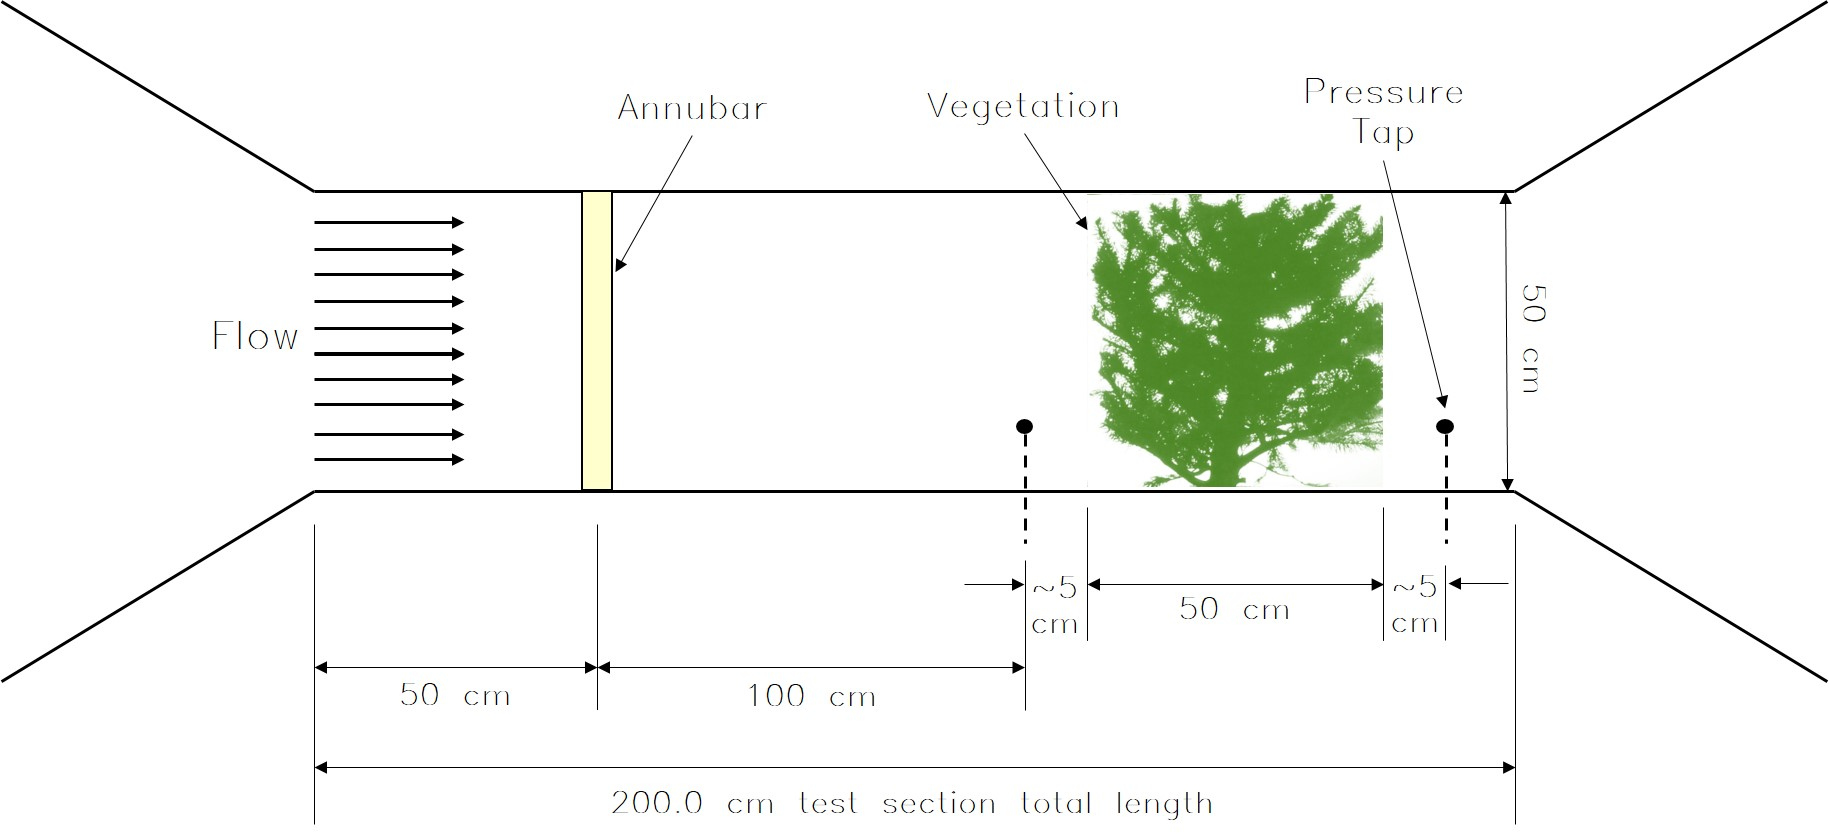
\includegraphics[width=1.0\linewidth]{Picture6.jpg}
	\caption{Schematic diagram of the wind-tunnel experimental setup (not to scale)}
	\label{fig:Windtun}
\end{figure}

\indent Once a set of measurements were taken at all nine fan speeds, the wind tunnel was shut off for a short amount of time (approx. 5 min), then proceeded by a repeated test. All wind tunnel tests were repeated three times for each vegetation configuration. The variances of the repeated tests' datasets for a given sample, cut, and position were compared using Hartley's F\textsubscript{Max} test. If it was found that the data sets were homogenous, then the data from the repeated tests were pooled together and averaged within the corresponding 30-second sampling time. \\
\indent An uncertainty analysis was also conducted for the wind tunnel measurements using propagation of error. The uncertainty of the pressure readings accounted for the calibration error (1.2 \%) and the reported accuracy error (0.15\% of the reading $\pm$ 0.02\% of the reading per \textdegree C). The uncertainty of the air density was determined from the standard error of the sampling data. Since the velocity and subsequently calculated drag coefficient were functions of the pressure, density, and free area fraction measurements, their respective uncertainties were determined through propagation of error.


\subsection{Water Displacement Testing to Determine the Volume and Solid Fraction (\textbeta)}
\label{ssec:headingscap}

The volume of vegetative solids was measured after a cut was made to the cubic vegetation sample. The remaining vegetative substance was separated into two groups of branches and leaves. Each group was packaged using a cloth mesh bag and thin wire. The wire volume and mass of the mesh bag and wire was measured before any displacement testing was conducted to determine only the vegetation material. Before submerging the packaged material, the dry weight of the sample was measured using a Mettler Toledo Jaguar load cell. After determining the dry weight, the packaged material was completely submerged in a bucket with a spout located approximately 3.8 \si{cm} from the top of the bucket. Before submerging the vegetation in water, the bucket was filled entirely with water, then allowed to drain at the lip of the spout to eliminate any additional displaced waterduring the test. Once the packaged vegetation was submerged, the displaced water was fed through the spout and into a glass beaker (Fig. \ref{fig:wdt}). Testing concluded once the flow through tubing stopped or exhibited infrequent drips. The collected beaker water was then poured into a 1000 ml graduated cylinder to determine the volume of solid vegetation.\\

\begin{figure} [!ht]
	\centering 	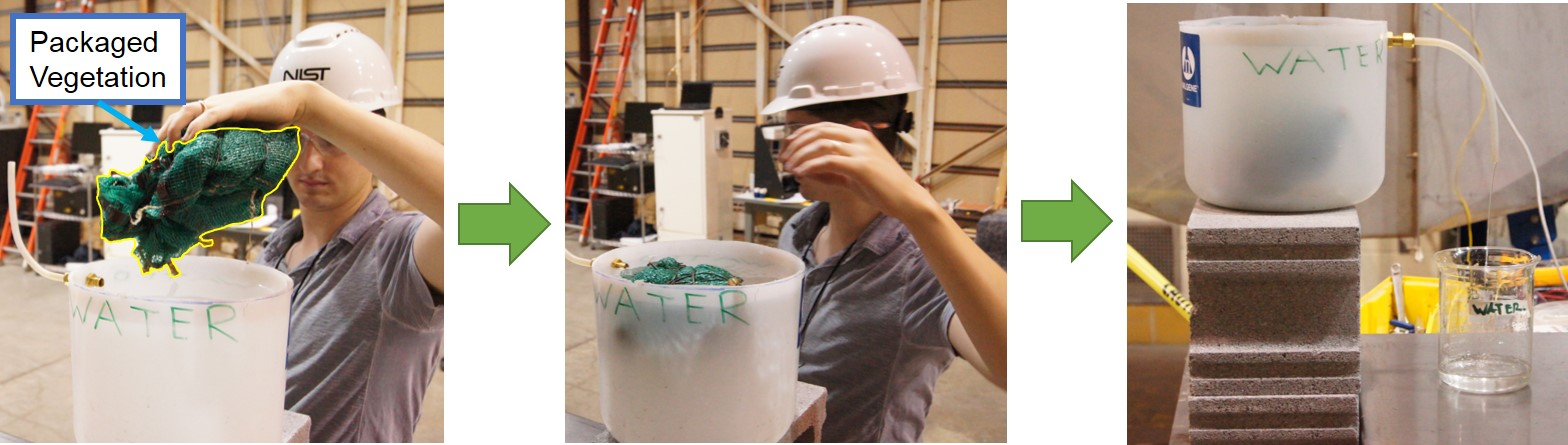
\includegraphics[width=1.0\linewidth]{Picture7.jpg}
	\caption{Procedure of the water displacement test}
	\label{fig:wdt}
\end{figure}

\indent Water displacement testing was conducted three times for each packaged vegetation. The weight of the vegetation was measured in between the displacement tests to account for any additional water that remained after the previous test. Once all volumes were determined for each vegetation cut, the solid fraction of the vegetation was calculated by dividing by the occupied space of the vegetation sample (0.5 \si{m} x 0.5 \si{m} x 0.5 \si{m} = 0.125 \si{m^{3}}). The uncertainty of the measured volume and solid fraction were also calculated from the propagation of error using the resolution of the Mettler Toledo load cell (0.005 kg), the resolution of the graduated cylinder used to measure the volume of the displaced water (5 ml), and the variance of the repeated displacement tests.

\pagebreak


%%%% Results section
\section{Results}
\label{sec:results}
The key result of this work was the drag coefficient determined through a combination of the results provided from each experiment. Additionally, a relationship between the absorption coefficient and solid fraction was also obtained from the image analysis and water displacement experiments.

\subsection{Vegetation Canopy Drag Coefficients}
\label{ssec:headingscap}
Table \ref{tab:SumTable} shows the average drag coefficient, and its respective uncertainty of each vegetation configuration categorized by species, cut, and position.

%For vegetation samples in which there were multiple cuts, it can be seen that the free area fraction increases with each cut iteration. The increase in the white fraction corresponds to the reduction of solid within the vegetation since each cut removes more of the canopy.

\begin{table}
\centering
\caption{Drag Coefficient Summary}
\label{tab:SumTable}
%\begin{adjustbox}{
  %addcode=
    %{\begin{minipage}{\width}}
    %{\caption{Summary Table}\label{tab:SumTable}\end{minipage}},
  %rotate=90,
  %center
%}
	%\centering
	\small
	\begin{tabular}{cccccccccccc}
	%\caption{Summary Table}	
			\hline
\textbf{Sample}	&	\textbf{Cut}	& 	\textbf{Position}	&	$C_{\rm D}$	&	\textbf{C\textsubscript{d} Uncertainty}	&	\\	\hline
		&		&			&				&						&	\\	
Bakers Blue Spruce	&	0	& 	A/C	&	3.35	&	0.02	&	\\	
	&		& 	B/D	&	3.10	&	0.01	&	\\	
	&	1	& 	A/C	&	3.40	&	0.01	&	\\	
	&		& 	B/D	&	3.29	&	0.02	&	\\	
	&	2	& 	A/C	&	2.82	&	0.01	&	\\	
	&		& 	B/D	&	2.74	&	0.01	&	\\	
	&	3	& 	A/C	&	2.35	&	0.02	&	\\	
	&		& 	B/D	&	2.26	&	0.01	&	\\	
	&		&		&		&		&	\\	
Blue Shag Eastern White Pine	&	0	& 	A/C	&	3.21	&	0.01	&	\\	
	&		& 	/BD	&	3.14	&	0.01	&	\\	
	&		&		&		&		&	\\	
Evergeen Distylium	&	0	& 	A/C	&	3.15	&	0.01	&	\\	
	&		& 	B/D	&	3.14	&	0.01	&	\\	
	&	1	& 	A/C	&	2.87	&	0.01	&	\\	
	&		& 	B/D	&	2.61	&	0.01	&	\\	
	&	2	& 	A/C	&	1.85	&	0.01	&	\\	
	&		& 	B/D	&	2.08	&	0.00	&	\\	
	&		&		&		&		&	\\	
Gold Rider Leyland Cypress	&	0	& 	A/C	&	3.18	&	0.01	&	\\	
	&		& 	B/D	&	3.09	&	0.01	&	\\	
	&	1	& 	A/C	&	3.29	&	0.01	&	\\	
	&		& 	B/D	&	3.33	&	0.01	&	\\	
	&	2	& 	A/C	&	2.57	&	0.01	&	\\	
	&		& 	B/D	&	3.25	&	0.01	&	\\	
	&	3	& 	A/C	&	2.97	&	0.01	&	\\	
	&		& 	B/D	&	3.84	&	0.01	&	\\	
			& 		&		&		&	\\	
Kimberley Queen Fern	&	0	& 	A/C	&	3.38	&	0.009	&	\\	
	&		& 	B/D	&	2.82	&	0.007	&	\\	
	&		&		&		&		&	\\		
Robin Red Holly	&	0	&	A/C	&	2.79	&	0.017	&	\\	
	&		&	B/D	&	2.66	&	0.005	&	\\	
	&	1	& 	A/C	&	2.68	&	0.003	&	\\	
	&		& 	B/D	&	1.91	&	0.006	&	\\	
	&	2	& 	A/C	&	3.03	&	0.003	&	\\	
	&		& 	B/D	&	2.34	&	0.011	&	\\	
	&	3	& 	A/C	&	1.85	&	0.015	&	\\	
	&		& 	B/D	&	1.64	&	0.012	&	\\	

		\hline
	\end{tabular}
%\end{adjustbox}

\end{table}

Figure~\ref{fig:DPvU(Overall)} shows the differential pressure measurements taken across the vegetation plotted against the free stream velocity. It can be observed that the differential pressure readings across a given velocity range are higher for vegetation configurations with higher free area fractions. By evaluating Eq.~(\ref{eq:Pressure}), the relationship between the dynamic pressure and the ratio between differential pressure measured across the vegetation and the product of the absorption coefficient and length can be seen in Fig. \ref{fig:DPoveraf(Overall)}. Despite exhibiting different geometric characteristics, Fig. \ref{fig:DPoveraf(Overall)} demonstrates that by incorporating the absorption coefficient and length, the pressure ratio moderately collapses suggesting a fairly consistent drag coefficient for the variety of vegetation canopies.


\begin{figure} [h]
	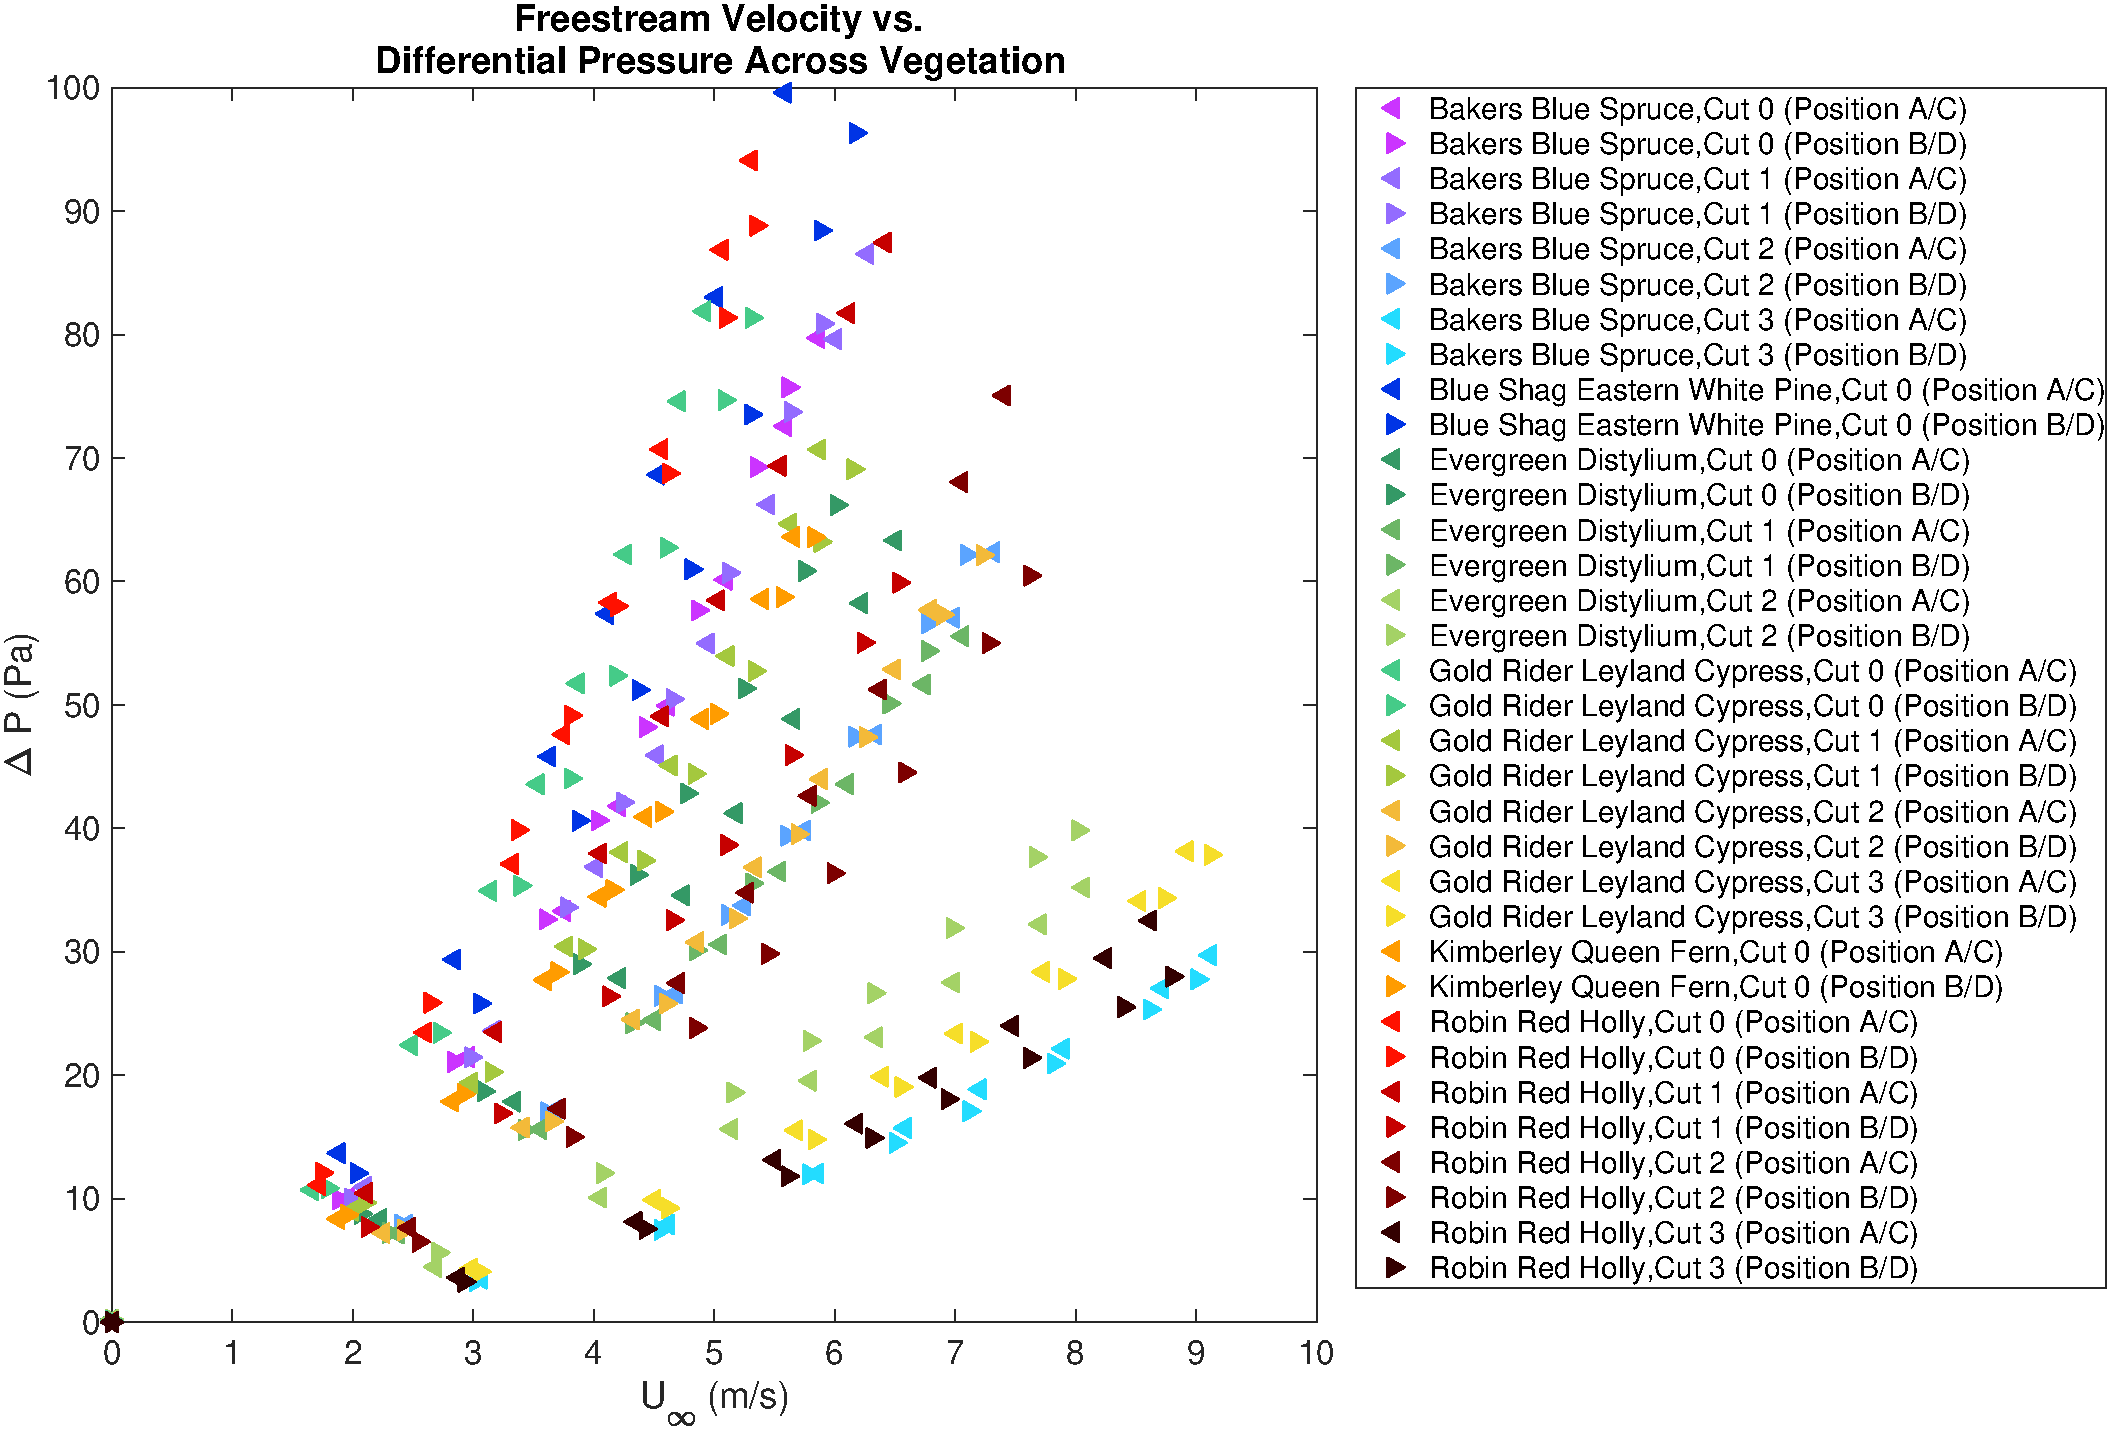
\includegraphics[width=\linewidth]{DPvU(Overall_Ave).pdf}
	\caption{Differential pressure measured across different vegetation samples subjected to various free stream velocities.}
	\label{fig:DPvU(Overall)}
\end{figure}

\begin{figure}[h]
	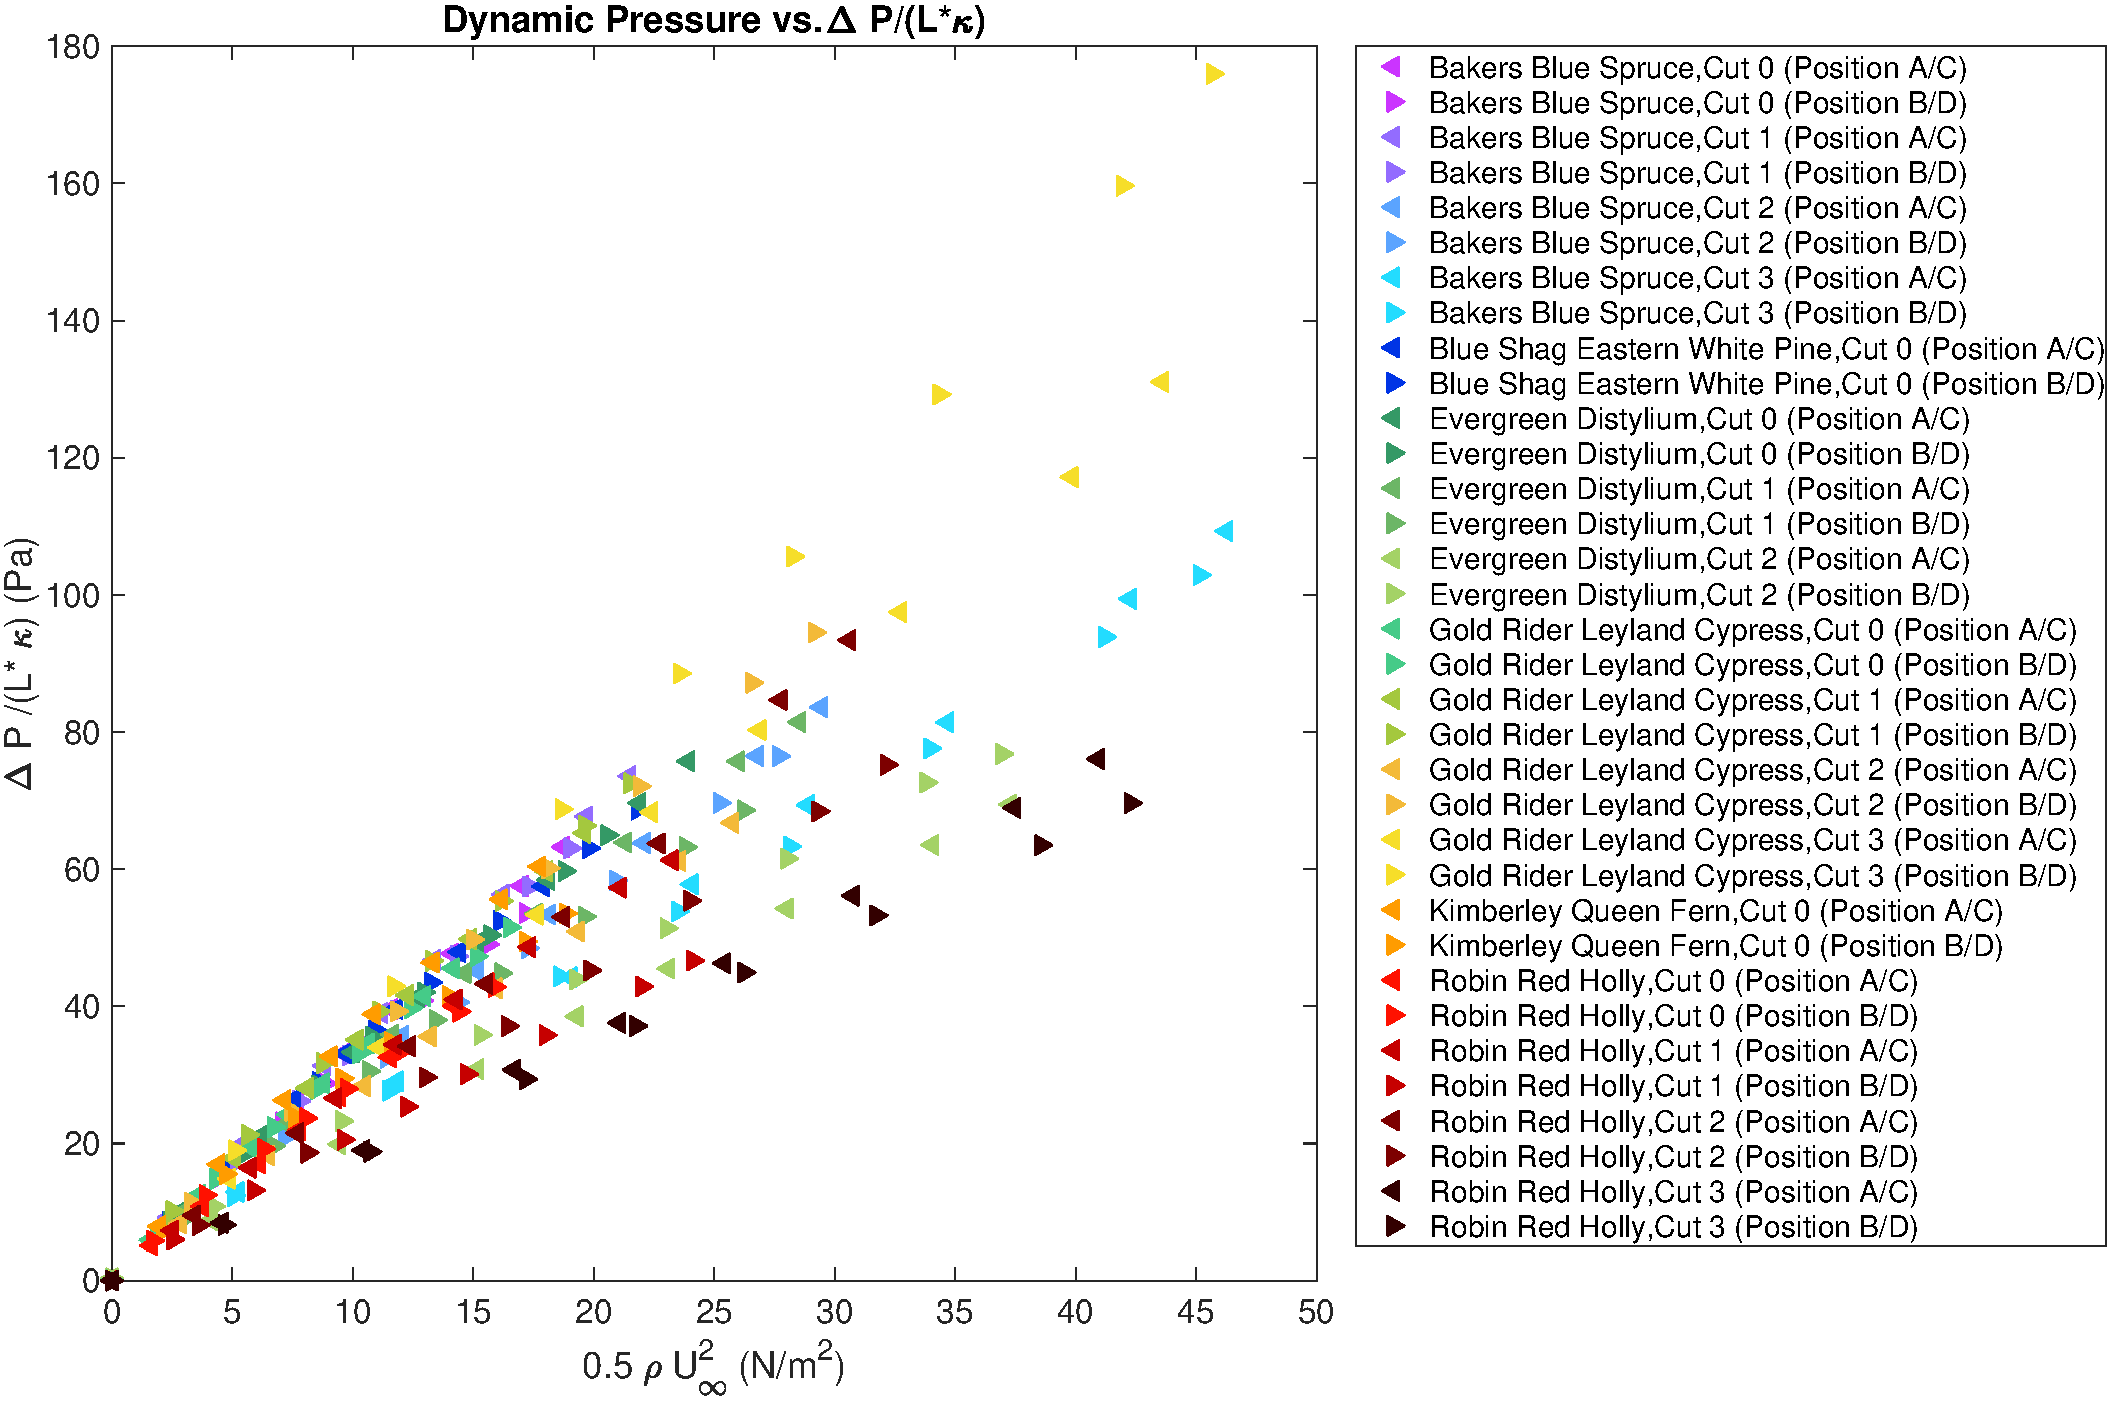
\includegraphics[width=\linewidth]{DPoveraf(Overall_Ave).pdf}
	\caption{Differential pressure across different vegetation samples over their respective ($\kappa L$) vs. dynamic pressureof.}
	\label{fig:DPoveraf(Overall)}
\end{figure}

\subsection{Relationship between the absorption coefficient $\kappa$ and solid fraction $\beta$ }

Figure \ref{fig:betavkappa} displays each samples' absorption coefficient plotted against their corresponding solid fractions. The markers presented in Figure \ref{fig:betavkappa} indicate the actual measured values while the dotted lines are a linear regression fit of the measured data. It can be observed that the absorption coefficient declines with the cut indicating that the removal of solid material from the vegetation after a cut increases the free area fraction, thus decreasing the absorption coefficient. Furthermore, Fig.~\ref{fig:betavkappa} also shows a discrepancy between the sample positions of the same cut. The difference in the absorption coefficients suggests that the area distribution within the canopy structure is inhomogeneously distributed. In other words, the original assumption that the vegetation canopy has a complex porous structure that is unevenly distributed and asymmetric is further supported by the discrepancy in the positioning data.

\begin{figure}[h]
	\centering 	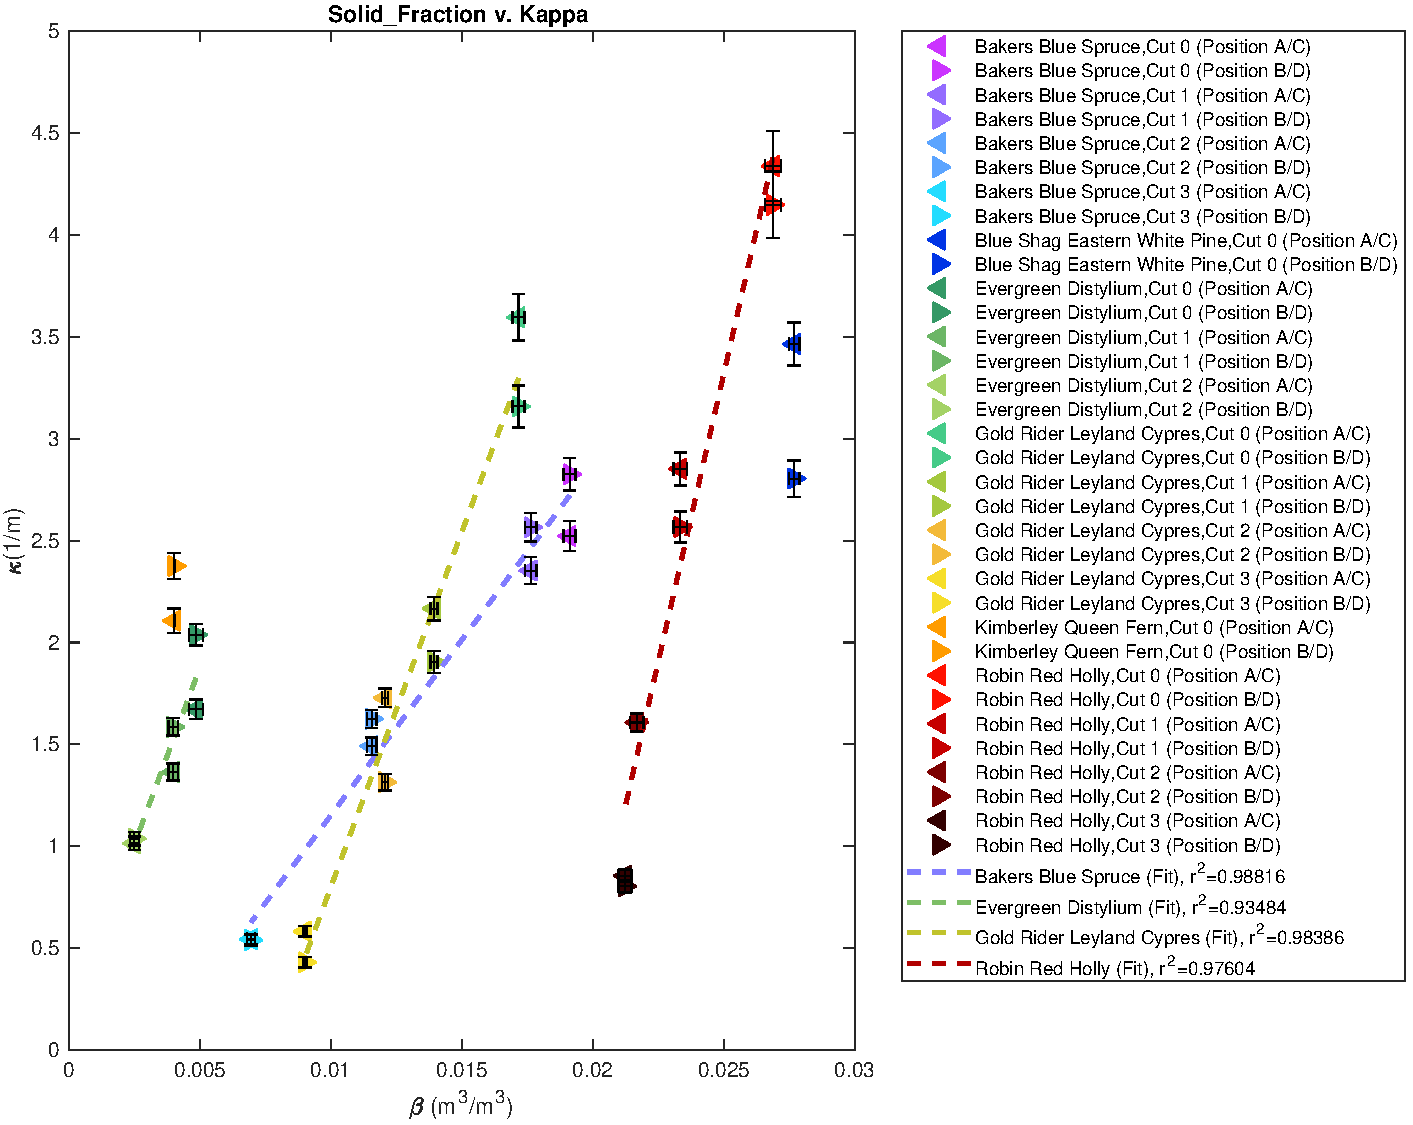
\includegraphics[width=0.8\linewidth]{Solid_FractionvKappa(Ave).pdf}
	\caption{Calculated absorption coeficients (\textkappa) plotted against their corresponding solid fractions (\textbeta) }
	\label{fig:betavkappa}
\end{figure}
\pagebreak

\section{Comparison Between Vegetation Data and Tube Bank Models}
\label{sec:comp}

A hydraulic resistant tube bank model was evaluated using similar geometric features (absorption coefficient and solid fraction) of the vegetation canopy samples to compare the drag coefficients of the two different configurations. Given the absorption coefficient and solid fraction an optimization code was applied to determine the tube bank configuration. The absorption coefficient and solid fraction values were slightly adjusted to accommodate row and number of tube integers. Once a tube bank configuration was obtained, the pressure loss across the tube banks were determined using I.E. Idelchik's hydraulic resistant tube bank model.  Eq.~\ref{eq:Pressure}, was then evaluated given the adjusted tube bank configuration parameters to determine the drag coefficient. It should be noted that in the calculation for the tube bank's drag coefficient, the distance L was assumed to be between rows alternative to across the entire vegetation.\\
%\indent The comparison between the vegetation sample's drag coefficient for a range of velocities and the drag coefficient of the corresponding tube bank is presented in Fig.\ref{fig:betavkappa}. It can be observed that by relatively matching the absorption coefficient, solid fraction, and average diameter of the vegetation sample, the tube bank model alligns fairly well with the measured data.


%%%%%%%%%%%%%%%%%%%%%%%%%%%%%%%%%%%%%%%%%%%%%%%%%%%%%%%%%%%%%%%%%%%%
%   Tables should appear after they are mentioned in the text.
%	Superscripted letters (a, b, c, etc.) should be used for table footnotes.
%%%%%%%%%%%%%%%%%%%%%%%%%%%%%%%%%%%%%%%%%%%%%%%%%%%%%%%%%%%%%%%%%%%%
%\begin{figure}[h]
%	\centering 	\includegraphics[width=0.5\linewidth]{Chrysanthemum.jpg}
%	\caption{This is the caption text \today}
%	\label{fig:Chrysanthemum}
%\end{figure}
%%%%%%%%%%%%%%%%%%%%%%%%%%%%%%%%%%%%%%%%%%%%%%%%%%%%%%%%%%%%%%%%%%%%
%   Figure references are “Fig. X”.
% 	“Figure X” is used at beginning of sentence.
% 	Figures should appear after they are mentioned in the text.
%	Figures must have embedded alternate text or “alt text” in order
%	to comply with Section 508 accessibility standards.
%%%%%%%%%%%%%%%%%%%%%%%%%%%%%%%%%%%%%%%%%%%%%%%%%%%%%%%%%%%%%%%%%%%%


\pagebreak

\section*{Acknowledgments}

\noindent Matthew Bundy and Artur Chernovksy of the National Fire Research Laboratory assisted in conducting these experiments and in processing the data.   \\
%%%%%%%%%%%%%%%%%%%%%%%%%%%%%%%%%%%%%%%%%%%%%%%%%%%%%%%%%%%%%%%%%%%%
%   Acknowledgments not required
%%%%%%%%%%%%%%%%%%%%%%%%%%%%%%%%%%%%%%%%%%%%%%%%%%%%%%%%%%%%%%%%%%%%

\section*{References}
\addcontentsline{toc}{section}{References}
\bibliographystyle{techpubs}
\bibliography{References}

%%%%%%%%%%%%%%%%%%%%%%%%%%%%%%%%%%%%%%%%%%%%%%%%%%%%%%%%%%%%%%%%%%%%
%   Please use the techpubs BibTeX style when compiling bibliography, or follow the instructions on tinyurl.com/techpubsnist to format your .bib / .bbl file appropriately.
%%%%%%%%%%%%%%%%%%%%%%%%%%%%%%%%%%%%%%%%%%%%%%%%%%%%%%%%%%%%%%%%%%%%
%%%%%%%%%%%%%%%%%%%%%%%%%%%%%%%%%%%%%%%%%%%%%%%%%%%%%%%%%%%%%%%%%%%%
%   Authors who have supplemental materials should submit them when submitting their manuscripts for review. Supplemental materials may include computer code or data files associated with the paper. A brief description of the supplemental material must be included in the paper. A DOI will be assigned to the supplemental material and inserted into the paper by the Information Services Office.
%%%%%%%%%%%%%%%%%%%%%%%%%%%%%%%%%%%%%%%%%%%%%%%%%%%%%%%%%%%%%%%%%%%%

\end{document}
